\chapter{Simulation-Based Calibration}
\label{sbc}

Simulation-Based Calibration (SBC) is a methodology designed to assess the calibration and correctness of Bayesian inference algorithms.
It was introduced by \textcite{cook_2006} and formalized by \textcite{talts_2020} as an approach to diagnose whether a probabilistic model, together with its inference engine, correctly reproduces the intended posterior distribution.
Unlike traditional model checking or convergence diagnostics, SBC focuses on the \emph{calibration} of the entire inference process, helping to determine whether an inference algorithm behaves as expected when the model is correctly specified.

\section{Theoretical Foundation}
\label{sec:theoretical_foundation}

The main idea of SBC is to use the rank statistic as a diagnostic measure.
For each simulation $i = 1, \dots, S$:

\begin{algorithm}[!ht]
    Sample $\theta_i \sim p(\theta)$\;
    Sample $y_i \sim p(y \mid \theta_i)$\;
    Obtain posterior samples $\{\theta_i^{(1)},\dots,\theta_i^{(L)}\} \gets \mathcal{A}(y_i)$\;
    Compute rank $R_i$ of $\theta_i$ among the posterior samples\;
    \caption{
        \textbf{Single iteration of the SBC procedure}.
        For each simulation, sample parameters from the prior, generate synthetic data, run inference, and compute the rank statistic.
    }
    \label{alg:sbc-iteration}
\end{algorithm}

Under the assumption that the inference algorithm, $\mathcal{A}$, correctly reproduces the posterior distribution $p(\theta \mid y)$, the rank statistic follows a discrete uniform distribution on $\{0, 1, \dots, L\}$.
Theorem \ref{thm:rank-uniformity} states and proves this result through an approach similar to the argument in Appendix B of \textcite{talts_2020}.
\begin{theorem}[Rank Uniformity Under Correct Posterior Inference]
    If the inference algorithm $\mathcal{A}$ used in Algorithm~\ref{alg:sbc-iteration} correctly reproduces the posterior distribution $p(\theta \mid y)$ for all $\theta$ and $y$, then the rank statistic $R_i$ produced by the SBC iteration is distributed uniformly on $\{0,1,\dots,L\}$.
    \label{thm:rank-uniformity}
\end{theorem}

\begin{proof}
    For simplicity, we will omit the indices in this proof.
    Now, without loss of generality, we can relabel all the posterior samples such that
    \[\theta^{(1)} \leq \theta^{(2)} \leq \dots \leq \theta^{(L)}.\]

    Then, we can write the probability mass function of the rank statistic as
    \begin{align*}
        p(r) & = \binom{L}{r} \int p(y, \theta)
                \cdot \lrp{\prod_{l=1}^{r} \int_{-\infty}^{\theta} p\lrp{\theta^{(l)}\mid \theta, y} d\theta^{(l)}}
                \cdot \lrp{\prod_{l=r+1}^{L} \int_{\theta}^{\infty} p\lrp{\theta^{(l)}\mid \theta, y} d\theta^{(l)}}
                d\theta dy \\
             & = \binom{L}{r} \int p(y, \theta)
                \cdot \lrp{\int_{-\infty}^{\theta} p\lrp{\theta^{(l)}\mid \theta, y} d\theta^{(l)}}^r
                \cdot \lrp{1 - \int_{-\infty}^{\theta} p\lrp{\theta^{(l)}\mid \theta, y} d\theta^{(l)}}^{L-r}
                d\theta dy.
    \end{align*}

    Since we condition on the data $y$, the posterior sample is independent of the generative parameter $\theta$, so
    \[p\lrp{\theta^{(l)}\mid \theta, y} = p\lrp{\theta^{(l)}\mid y}.\]

    Also, using that $p(y, \theta) = p(\theta \mid y)\cdot p(y)$ we can rewrite
    \begin{align*}
        p(r) & = \binom{L}{r} \int p(y, \theta)
                \cdot \lrp{\int_{-\infty}^{\theta} p\lrp{\theta^{(l)}\mid \theta, y} d\theta^{(l)}}^r
                \cdot \lrp{1 - \int_{-\infty}^{\theta} p\lrp{\theta^{(l)}\mid \theta, y} d\theta^{(l)}}^{L-r}
                d\theta dy \\
             & = \binom{L}{r} \int p(y) \int p(\theta \mid y)
                \cdot \lrp{\int_{-\infty}^{\theta} p\lrp{\theta^{(l)}\mid y} d\theta^{(l)}}^r
                \cdot \lrp{1 - \int_{-\infty}^{\theta} p\lrp{\theta^{(l)}\mid y} d\theta^{(l)}}^{L-r}
                d\theta dy.
    \end{align*}

    Since the algorithm correctly reproduces the posterior distribution, we have
    \[p\lrp{\theta^{(l)} \mid y} = p(\theta \mid y).\]

    Now, define
    \[u = \int_{-\infty}^{\theta} p(t \mid y) dt = F_y(\theta) \implies u \in [0, 1] \land du = p(\theta \mid y) d\theta,\]
    \noindent which allows us to change the variables in the integral. Then
    \begin{align*}
        p(r) & = \binom{L}{r} \int p(y) \cdot \int_0^1 u^r \cdot \lrp{1 - u}^{L-r} du dy \\
             & = \dfrac{L!}{r! \cdot (L - r)!} \int p(y) \cdot \dfrac{r! \cdot (L - r)!}{(L + 1)!} dy \\
             & = \dfrac{1}{L + 1} \int p(y) dy \\
             & = \dfrac{1}{L + 1},
    \end{align*}

    \noindent which is consistent with a uniform distribution over the $L + 1$ possible ranks of the set $\{0, 1, \dots, L\}$.
\end{proof}

In practice, Theorem \ref{thm:rank-uniformity} states that by repeating this process across $S$ simulations, we can plot and see visually or test statistically whether the computed ranks are uniformly distributed to validate the calibration of the inference process.
Figure \ref{fig:sbc_workflow} shows the workflow of this validation.

\begin{figure}[!ht]
    \centering
    \begin{tikzpicture}[
        node distance=0.9cm,
        >=Latex,
        thick,
        process/.style={
            draw,
            rounded corners,
            minimum width=4cm,
            minimum height=1cm,
            align=center,
            font=\small,
            fill=#1!15
        },
        process/.default=blue,
        decision/.style={
            diamond,
            aspect=2.2,
            draw,
            align=center,
            inner sep=1pt,
            fill=yellow!15,
            font=\small
        }
    ]

        % ---- Nodes ----
        \node[process=magenta]
            (start)  {Set $i  = 0$};
        \node[process=blue,   below=of start]
            (sample)  {Update i = i + 1 \\ Sample $\theta_i \sim p(\theta)$};
        \node[process=green,  below=of sample]
            (simulate) {Simulate $\boldsymbol{y_i} \sim p(\boldsymbol{y} \mid \theta_i)$};
        \node[process=orange, below=of simulate]
            (infer) {Infer $p(\theta \mid \boldsymbol{y_i})$};
        \node[process=red,    below=of infer]
            (rank) {Compute rank of $\theta_i$};
        \node[process=cyan,   below=of rank]
            (store) {Store rank $r_i$};
        \node[decision, below=of store]
            (check) {$i = S$ ?};
        \node[process=gray,   right=2cm of check, text width=4.2cm]
            (aggregate) {Check uniformity \\ of $\{r_i\}_{i=1}^S$};

        % ---- Arrows ----
        \draw[->] (start) -- (sample);
        \draw[->] (sample) -- (simulate);
        \draw[->] (simulate) -- (infer);
        \draw[->] (infer) -- (rank);
        \draw[->] (rank) -- (store);
        \draw[->] (store) -- (check);

        % Decision arrows
        \draw[->] (check.east) -- node[above]{yes} (aggregate.west);
        \draw[->, bend left=40] (check.west) to node[left]{no} (sample.west);

    \end{tikzpicture}
    \caption{
        \textbf{SBC workflow}.
        For each simulated dataset, we generate $\theta_i$, simulate data $y_i$, infer the posterior, and check whether ranks of $\theta_i$ are uniformly distributed.
    }
    \label{fig:sbc_workflow}
\end{figure}


\section{Uniformity and Deviations}
\label{sec:uniformity_deviations}

As mentioned in the previous section, if the inference algorithm is unbiased and correctly implemented, the histogram of ranks should be approximately flat.
Bias and under/overdispersion can be identified looking into the histogram, Empirical Cumulative Distribution Function (ECDF) or ECDF difference plots of the computed ranks.
Figure \ref{fig:sbc_viz} shows how common deviations can be identified in the ECDF difference plot.
For this example, we ran $2560$ simulations, each generating $\mu \sim \mathcal{N}(0, 1)$ and sampling $10$ points from a distribution $\mathcal{N}(\mu, 1)$.
The inference process ran $100$ iterations of warm-up and $127$ iterations with posterior sampling.

\begin{figure}[htbp]
    \centering
    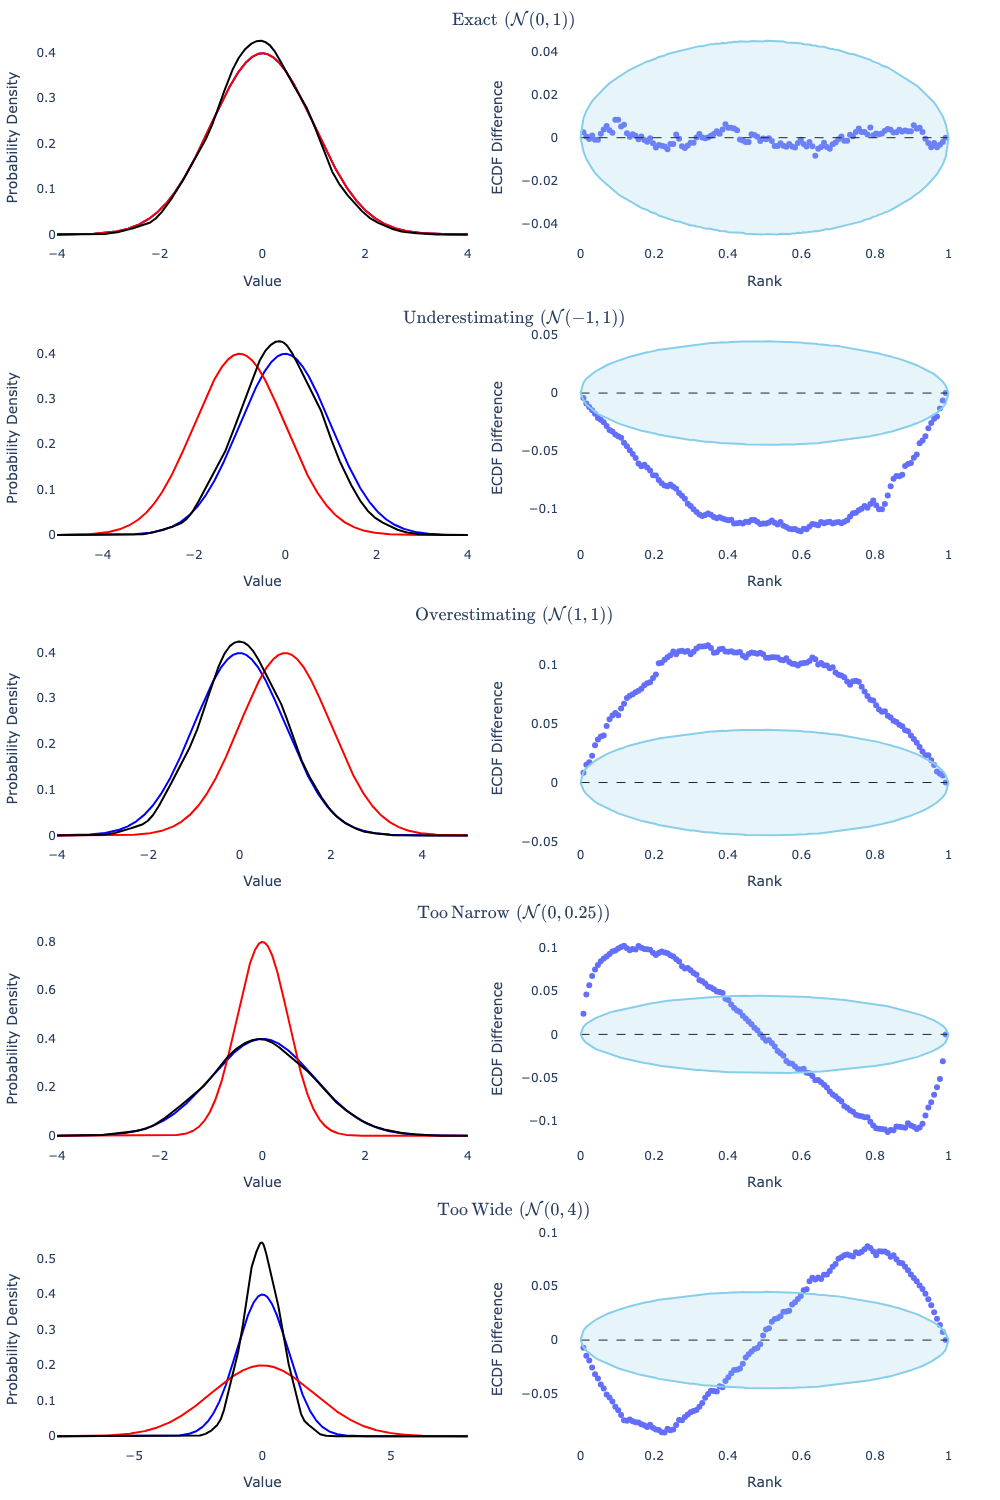
\includegraphics[width=0.85\linewidth]{figures/sbc_visualization.png}
    \caption{
        \textbf{SBC applied on synthetic data}.
        The true $\mu$ distribution is given by the blue distribution.
        The red distribution was set as data conditional distribution on inference process during the SBC validation.
        The black distribution is the kernel density estimate (KDE) for the $\mu$ posterior.
        The second column shows the ECDF difference plot for the normalized rank distribution.
        Under a well calibrated model, this ECDF is expected to be a straight line from $(0, 0)$ to $(1, 0)$.
    }
    \label{fig:sbc_viz}
\end{figure}

As we can see in Figure \ref{fig:sbc_viz}, a bias in the posterior reflects on a U-shape or an inverted U-shape in the ECDF differences plot.
On the other hand, under/overdispersion in the posterior results in a S-shape.


\section{Computational and High Dimensional Considerations}
\label{sec:computational_considerations}

As illustrated in Figure \ref{fig:sbc_workflow}, SBC can be computationally expensive, as it requires repeated posterior inference for many synthetic datasets.
This cost can be mitigated through parallelisation, since each inference run is independent.
Despite the high computational cost, performing SBC early in the modelling process allows for detection of coding mistakes or conceptual errors before substantial resources are spent on large-scale analyses.
For this reason, it is recommended that SBC be considered as part of the Bayesian model development process, rather than an afterthought, as emphasised by \textcite{gelman_2020}.

These computational challenges become even more pronounced in high-dimensional models, where a large number of parameters must be assessed simultaneously.
Applying SBC independently to each parameter is conceptually straightforward but has a huge cost.
To reduce this cost, the workflow in Figure \ref{fig:sbc_workflow} can be extended to high dimensional models by just taking $\theta$ as a $d$-dimensional vector.
For each component of $\theta$, rank statistics can be computed and stored across simulations, and their empirical distributions can then be checked for uniformity.
While this approach increases storage and computational demands, it provides a systematic way to diagnose inference quality even in complex, high-dimensional settings.


\section{Experimental Design}
\label{sec:sbc_experimental_design}

All SBC experiments were designed to represent the typical format of a \textit{Brasileirão Série A} season.
For each model, $S = 500$ synthetic datasets were generated, each comprising $n = 20$ teams competing in a double round-robin tournament with $380$ matches.

The inference process uses Stan \cite{carpenter_2017} via the CmdStanPy interface \cite{cmdstanpy}.
Each simulation was run with 4 parallel chains, 1,000 warm-up iterations, and 1,000 sampling iterations per chain, yielding 4,000 posterior samples per simulation.
The sampler was configured with an adaptation target acceptance probability of $\delta = 0.95$ and a maximum tree depth of 10.

For each simulation $i$, the true parameter values $\boldsymbol{\theta}_i$ were sampled from the prior distributions specified in the model.
Synthetic data $\mathbf{y}_i$ were generated according to the likelihood, and posterior samples $\{\boldsymbol{\theta}_i^{(1)}, \ldots, \boldsymbol{\theta}_i^{(L)}\}$ were obtained via Markov Chain Monte Carlo (MCMC).
The normalized rank of each true parameter value among its posterior samples was recorded.
Under correct posterior inference, these ranks should follow a uniform distribution on $[0, 1]$, as established in Theorem~\ref{thm:rank-uniformity}.

Since there are a lot of models, with many parameters, to evaluate, we use a systematic approach to identify potential miscalibrations.
For each parameter in a model, we compute the ECDF difference plot and check whether any point falls outside the 95\% confidence envelope.
If at least one point lies outside this envelope, that parameter is flagged, and we record the total number of points outside the envelope for that parameter.
Aggregating across all parameters of a model, we obtain two summary statistics: the total number of flagged parameters (``Flags'') and the cumulative count of points outside the confidence envelopes (``Points Out'').
A model with many flagged parameters or a large cumulative count suggests potential miscalibration.
However, under correct calibration, we expect approximately 5\% of parameters to be flagged by chance alone, and minimal deviations may still occur due to the inherent randomness of the simulations.

